% !TeX root = ../presentation.tex

\section*{Introducción}
%----------------------------------------------------------------------------------
\begin{frame}{Motivación}
\begin{alertblock}{Metasupeficies plasmónicas para biosensado}
    \begin{itemize}%[<+->]
    \itemsep9pt
    \item Arreglos bidimensionales de \textbf{nanoestructuras metálicas} (meta-átomos) soportadas por un sustrato.
    \end{itemize}
    \end{alertblock}

    \begin{center}
  	  \begin{tikzpicture}[node distance=0em and .75cm,font=\small]
%
	   \node[flowbox] (bio) {\fbtitle{Estudio teórico}\vphantom{yÖ}
	    \nodepart{two}
        \begin{minipage}{.25\textwidth} \begin{itemize}
			\item Condiciones ideales
			\item Periodicidad
        \end{itemize}\end{minipage}
    };
%
		\node[below=of bio] (nanofoto) {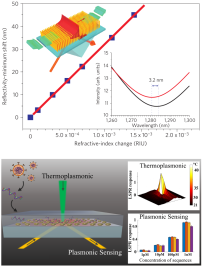
\includegraphics[scale = .6]{kabashin-quin.png}};
		\node[right=of nanofoto] (nanofoto) {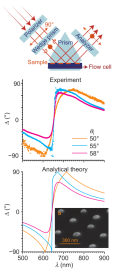
\includegraphics[scale = .6]{kaell.png}};
%
    \end{tikzpicture}
    \end{center}
%
% 	\begin{textblock*}{1cm}(0cm,-4.75cm)
% 	\includegraphics[scale=.1]{img/1-Intro/SPP-3D-noTags}
% 	\end{textblock*}
%
% \footnotetext[1]{\tiny\fullcite{mun2015nanobiosensors}}
% \footnotetext[2]{\tiny\fullcite{svedendahl2009refractometric}}
% \footnotetext[3]{\tiny\fullcite{estevez2014trends}}
\end{frame}
